\subsection{Example}\label{sec:example}


As an example, let us consider the pipeline template \tChartFunction in \cref{sec:example}.

In this example all the policies referenced are detailed in table \ref{tab:anonymization}.
We assume that the data owner is the Connecticut Prison (CTP) and that this facility has a partnership with two others, namely New York Prison and New Hampshire Prison.

The first stage is responsible for data anonymization. The  policy annotation \P{i}, associated with the first stage,
specifies three degree of anonymization : \emph{none}, \emph{partial}, and \emph{full}.
During service execution, the policy is assessed:
if the service profile match with the data owner, \P{1} is satisfied and the data is not anonymized;
if the service profile match with a partner of the owner, \P{2} is satisfied and the data is partially anonymized;
if the service profile doesn't match with a partner nor with the owner, \P{3} is satisfied and the data is fully anonymized.

The second stage is responsible for data enrichment. The policy annotation $p$, associated with the second stage,

The third stage, responsible for data analysis and statistics, adopts policies analogous to the first stage. The logic remains consistent:
if the service profile match with the data owner, \P{1} is satisfied and the data computation is made on non anonymized data;
if the service profile match with a partner of the owner, \P{2} is satisfied and the data computation is made on partially anonymized data;
if the service profile doesn't match with a partner nor with the owner, \P{3} is satisfied and the data computation is made on fully anonymized data.
The fourth stage is responsible for machine learning tasks:
policy \p{4} applies, thus we always aim to anonymize the dataset to avoid any personal identifiers entering into the machine learning algorithm/model.
The fifth stage is responsible for storing data. As stated in policy annotation \P{5}, if the service is located in the facility itself, the data will not be anonymized.
If the service is located in a partner region, the data will be partially anonymized.

The sixth stage is responsible for data visualization. As stated in policy annotation \P{6}, if the user is member of the facility itself, the data will not be anonymized.
If the user is member of a partner facility, the data will be partially anonymized.
If the user is not member of the facility nor a partner, the data will be fully anonymized.





\begin{table*}[ht!]
  \centering
  \bgroup
  \def\arraystretch{1.5}
  \begin{tabular}{c|c||l}
    \textbf{Policy} & \textbf{Service} & \textbf{Anonymization}                                                                                \\ \hline

    $\p{1}$         & \s{1}            & \policy{$\langle service,owner=``CTP"\rangle$}{dataset}{READ}{ANY}{\varnothing}                       \\
    $\p{2}$         & \s{1}            & \policy{$\langle service,owner=partner(``CTP") \rangle$}{dataset}{READ}{ANY}{light\_anonymization}    \\
    $\p{3}$         & \s{1}            & \policy{$\langle service,owner=``Connecticut Prison"$}{dataset}{READ}{ANY}{full\_anonymization}       \\
    $\p{4}$         & \s{4}            & \policy{ANY}{dataset}{READ}{ANY}{full\_anonymization}                                                 \\
    $\p{5}$         & \s{5}            & \policy{$\langle service,region=``FACILITY"\rangle$}{dataset}{WRITE}{ANY}{none}                       \\
    $\p{6}$         & \s{5}            & \policy{$\langle service,region=``{CT,NY,NH}"\rangle$}{dataset}{WRITE}{ANY}{light\_anonymization}     \\
    $\p{7}$         & \s{6}            & \policy{$\langle,user,role=   ``Connecticut Prison Officer"$}{dataset} {READ}{ANY}{none}              \\
    $\p{7}$         & \s{6}            & \policy{$\langle,user,role=   ``Partener Prison Officer"$}{dataset} {READ}{ANY}{light\_anonymization} \\
    $\p{8}$         & \s{6}            & \policy{$\langle,user,role=   ``Any"$}{dataset} {READ}{ANY}{full\_anonymization}                      \\
  \end{tabular}
  \egroup
  \caption{Anonymization policies}
  \label{tab:anonymization}
\end{table*}

\begin{figure}[ht!]
  \centering
  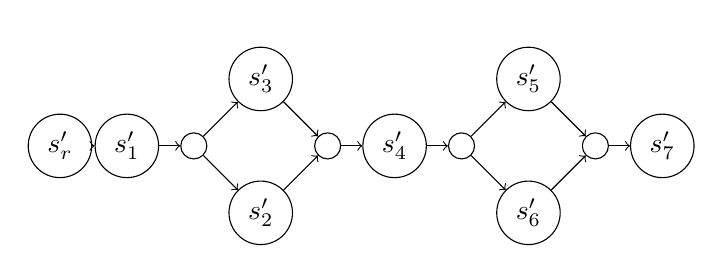
\begin{tikzpicture}[scale=0.85]
    \node[draw, circle] (node1) at (0,0) {$s^\prime_r$};
    \node[draw, circle] (node2) at (1,0) {$s^\prime_1$};
    \node[draw, circle] (node3) at (2,0) {$\timesOperator$};
    \node[draw, circle] (node4) at (3,-1) {$s^\prime_2$};
    \node[draw, circle] (node5) at (3,1) {$s^\prime_3$};
    \node[draw, circle] (node6) at (4,0) {$\timesOperator$};
    \node[draw, circle] (node65) at (5,0) {$s^\prime_4$};
    \node[draw, circle] (node7) at (6,0) {$\plusOperator$};
    \node[draw, circle] (node8) at (7,1) {$s^\prime_5$};
    \node[draw, circle] (node9) at (7,-1) {$s^\prime_6$};
    \node[draw, circle] (node10) at (8,0) {$\plusOperator$};
    \node[draw, circle] (node11) at (9,0) {$s^\prime_7$};
    % Text on top
    \node[above] at (node1.north) { \footnotesize$\instanceChartAnnotation$};
    \node[above] at (node2.north) { \footnotesize$\instanceChartAnnotation$};
    \node[above] at (node3.north) {};
    \node[above] at (node4.north) { \footnotesize$\instanceChartAnnotation$};
    \node[above] at (node5.north) { \footnotesize$\instanceChartAnnotation$};
    \node[above] at (node65.north) { \footnotesize$\instanceChartAnnotation$};
    \node[above] at (node8.north) { \footnotesize$\instanceChartAnnotation$};
    \node[above] at (node9.north) { \footnotesize$\instanceChartAnnotation$};
    \node[above] at (node11.north) { \footnotesize$\instanceChartAnnotation$};
    % Connection
    \draw[->] (node1) -- (node2);
    \draw[->] (node2) -- (node3);
    \draw[->] (node3) -- (node4);
    \draw[->] (node3) -- (node5);
    \draw[->] (node5) -- (node6);
    \draw[->] (node4) -- (node6);
    \draw[->] (node6) -- (node65);
    \draw[->] (node65) -- (node7);
    \draw[->] (node7) -- (node8);
    \draw[->] (node7) -- (node9);
    \draw[->] (node8) -- (node10);
    \draw[->] (node9) -- (node10);
    \draw[->] (node10) -- (node11);
  \end{tikzpicture}
  \caption{Service composition instance}
  \label{fig:service_composition_instance}
\end{figure}
